%!TEX root = ../fbi.tex

\section{Correlation functions}

When in the quasi-1D cylinder geometry, the tensor network 
wavefunction can be viewed as an MPS, and correlation functions can be 
analyzed using the transfer matrix of the MPS. \brayden{cite some MPS 
paper}. In this case, we find that the leading eigenvalue of the 
transfer matrix is non-degenerate, so all correlation functions decay 
exponentially down the cylinder for a fixed $L$. Furthermore, we find 
that the correlation length approaches a finite constant as we 
increase $L$, as shown in Figure \ref{fig:TMS}.

This 1D correlation length bounds all correlations stretching along 
the cylinder, but it is possible that placing the state on a cylinder 
- which explicitly breaks the rotational symmetry of the honeycomb 
lattice - leads to anisotropic correlations, even in the large $L$ 
limit. By looking at explicit short-distance correlation functions 
$\ev{b_i^{\dagger} b_j}$ and $\ev{n_i n_j}$, we see that instead the 
rotational symmetry is restored in the large $L$ limit. Our maximum 
cylinder circumference $L=10$ is several times larger than the 
measured correlation length $\xi \approx 3.2$.

\begin{figure}[hbtc]
	\centering
	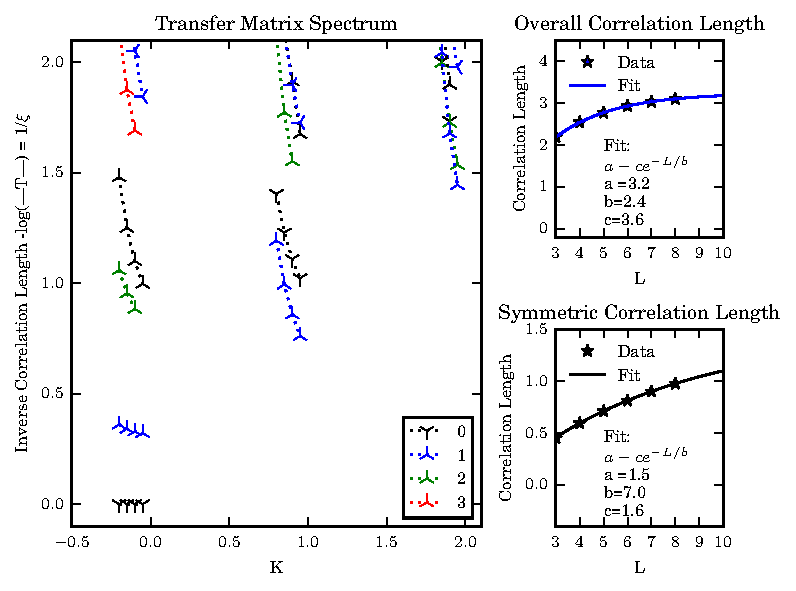
\includegraphics[width=\columnwidth]{TransferMatrixSpectrum_big.pdf}
	\caption{Placeholder for plots showing correlation bounds.}
	\label{fig:TMS}
\end{figure}

\begin{figure}[hbtc]
	\centering
	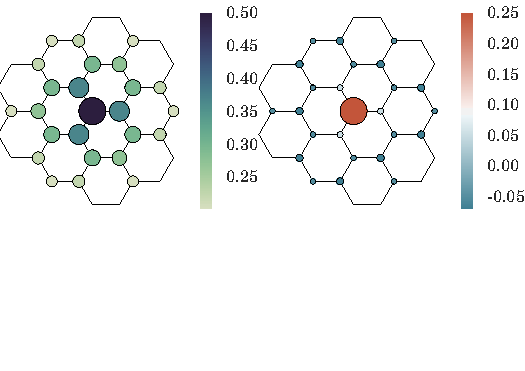
\includegraphics[width=0.6\columnwidth]{ShortDistanceCorrelations.pdf}
	\caption{Placeholder for 2D short distance correlation plot.}
	\label{fig:ShortCorr}
\end{figure}

\bela{Show that everything agrees with MC results, as far as those are 
available.}